\documentclass[review]{elsarticle}

\usepackage{lineno,hyperref}
\usepackage{graphicx}
\modulolinenumbers[5]

\journal{Expert Systems with Applications}

%%%%%%%%%%%%%%%%%%%%%%%
%% Elsevier bibliography styles
%%%%%%%%%%%%%%%%%%%%%%%
%% To change the style, put a % in front of the second line of the current style and
%% remove the % from the second line of the style you would like to use.
%%%%%%%%%%%%%%%%%%%%%%%

%% Numbered
%\bibliographystyle{model1-num-names}

%% Numbered without titles
%\bibliographystyle{model1a-num-names}

%% Harvard
%\bibliographystyle{model2-names.bst}\biboptions{authoryear}

%% Vancouver numbered
%\usepackage{numcompress}\bibliographystyle{model3-num-names}

%% Vancouver name/year
%\usepackage{numcompress}\bibliographystyle{model4-names}\biboptions{authoryear}

%% APA style
%\bibliographystyle{model5-names}\biboptions{authoryear}

%% AMA style
%\usepackage{numcompress}\bibliographystyle{model6-num-names}

%% `Elsevier LaTeX' style
\bibliographystyle{elsarticle-num}
%%%%%%%%%%%%%%%%%%%%%%%

\begin{document}

\begin{frontmatter}

\title{Origin based Association Rule Mining using multiple MASP tree\tnoteref{mytitlenote}}
\tnotetext[mytitlenote]{Fully documented templates are available in the elsarticle package on \href{http://www.ctan.org/tex-archive/macros/latex/contrib/elsarticle}{CTAN}.}

%% Group authors per affiliation:
\author{Elsevier\fnref{myfootnote}}
\address{Radarweg 29, Amsterdam}
\fntext[myfootnote]{Since 1880.}

%% or include affiliations in footnotes:
\author[mymainaddress,mysecondaryaddress]{Elsevier Inc}
\ead[url]{www.elsevier.com}

\author[mysecondaryaddress]{Global Customer Service\corref{mycorrespondingauthor}}
\cortext[mycorrespondingauthor]{Corresponding author}
\ead{support@elsevier.com}

\address[mymainaddress]{1600 John F Kennedy Boulevard, Philadelphia}
\address[mysecondaryaddress]{360 Park Avenue South, New York}

\begin{abstract}
Association rule learning is a rule-based machine learning method for discovering interesting relations between variables in large databases.
\end{abstract}

\begin{keyword}
data-mining \sep Association Rule Mining \sep frequent-itemset mining 
\end{keyword}

\end{frontmatter}

\section{Introduction}
Association rule mining is a rule-based machine learning procedure to find interesting patterns in the transaction database based on individual and conditional frequencies. In the traditional approach, two steps are involved in generating rules. First, generate all frequent itemsets and pruned non-frequent ones and then in the second stage rules are derived from those frequent itemsets. An association rule e.g. \{bread, milk\} $\Rightarrow$ \{butter\} in market basket analysis means if one purchase bread and milk together it is highly likely that they will also buy butter. Apart from market basket analysis, association rule mining is useful in intrusion detection, bioinformatics, and many other applications.

In 2014 O. M. Soyal \cite{oldmasp} proposed a new approach to extract mostly associated sequential patterns (MASPs) using less computational resources in terms of time and memory while generating a long sequence of patterns that have the highest co-occurrence.

This approach may produce different outcomes if we change the order of items in transactions. We propose an approach which is order independent. An association rule of the form A $\Rightarrow$ B must satisfy the threshold support and threshold confidence i.e. probability of occurrence of A and B together must surpass threshold support, and the probability of occurrence of B in transactions containing A must be greater than or equal to threshold confidence. It means, to calculate support and confidence, it is required to traverse complete transaction database. To generate all rules containing a particular item x it is reasonable to ignore all transactions(for calculating support and confidence) that come before the transaction in which that particular item appears for the first time. Embedding these two changes to the Omer M. Soyal \cite{oldmasp} approach is the basis of our research.

\section{Related works}
In 1994 R. Agrawal, et al. published non-trivial algorithm(Apriori) \cite{fastapriori} for finding association rules in large databases of the sales transaction. Apriori algorithm produces association rules in two steps. First generates all frequent itemsets(prune non-frequent candidate itemsets) and then make rules from those itemsets. This algorithm first finds frequent itemsets of length one then frequent itemsets of length 2 using frequent itemsets of length 1 and so on until generation of all frequent itemsets. This algorithm gave the better result than the previously known fundamental algorithms AIS \cite{ais}, SETM \citep{setm}. In 1996 Fukuda, et al. \cite{2darules} proposed an approach to find two-dimensional association rules. A state in this scenario is of the form ((X, Y) $\in$ P) $\Rightarrow$ (Z = z) where X and Y are numeric attributes, P is a subspace of 2-D plane, and Z is boolean attribute i.e. z can be either true or false. E.g. (Age $\in$ [30, 50] $\wedge$ Balance $\in$ [10$^{5}$, 10$^{6}$]) $\Rightarrow$ (CardLoan = yes). It means if a bank user age and balance lies in the given subspace it is very likely that they will use card loan. This approach works for specific types of structured data. R. Feldman, et al.(1997) \cite{massociation} introduced the notion of maximal association rules. These are the rules extracted from frequent maximal itemsets. Frequent maximal itemsets are those itemsets which appear just once among all transactions. It is useful in finding association rules containing negated attributes. As an example a rule \{milk, $\neg$bread\} $\Rightarrow$ \{$\neg$butter\} contains negated attributes. It means if a user purchases milk but not bread then the probability that the user will not buy butter is very high. This approach helps to capture inference rules which might be lost using regular associations. Till now items in transaction databases were treated uniformly. In 1998 C.H. Cai, et al. \cite{weightedassociation} gave an approach to find association rules which take into account weight(importance) of items in transaction databases. FP-Growth algorithm(2000) \cite{fpgrowth} also take two steps. The second phase is same as apriori. FP-Growth does not generate candidate frequent itemsets. First, it creates a tree(FP-Tree) and then finds frequent itemsets. This algorithm is about an order of magnitude faster than the Apriori algorithm. Lin, Weiyang, et al. \cite{Lin2002} proposed an approach that uses association rule mining for collaborative recommender systems. This approach does not require threshold support value. Instead, based on the number of rules(given) to be generated, threshold support is decided by the system. Thus it reduced the running time and produced enough rules for good recommendation performance. In 2004 F. Conen, et al. \cite{ptree} proposed two structures(T-Trees and P-Trees) which offer improvement concerning storage and execution time. In 2005 K. G. Srinivasa, et al. \cite{genetic} took advantage of genetic algorithms principles to generate large itemsets within dynamic transaction database. Their algorithm was better than the pre-existing FUP and E-Apriori concerning execution time and scalability. If transaction database is static, then life will be easy. In other scenario transaction database keeps on changing at high speed leading to change in data distribution. Hence it will be difficult to apply previously mentioned Association Rule Mining techniques. Jiang, et al.(2006) \cite{dynamicarm} came up with an approach to overcome this difficulty. In the same year G. Chen, et al. \cite{classify} used association rule mining for solving classification problems. It gave satisfactory results when compared to existing classification algorithms like C4.5, CBA, SVM, NN. Modification in traditional algorithm(apriori) was done \cite{bookrecommend} for building book recommendation system based on the data obtained from historical data of university library. Association rules having low support and high confidence are exception rules. In 2008 D. Taniar, et al. \cite{exceptionrules} proposed a new approach to finding exception rules. First, generate candidate exception rules and based on exceptionality measure obtain final ruleset. The quality of association rules depends on the threshold value of support and confidence. R.J. Kuo, et al.(2011) \cite{swarmarm} proposed an approach to find best threshold values which can produce quality rules. It gave promising results when compared to the genetic algorithm. Cloud computing provides an efficient and cheap way to store and analyze data. In 2011 L. Li, et al. \cite{cloudarm} proposed an effective strategy to perform association rule mining(frequent itemset mining) in cloud computing environment. Apriori \cite{fastapriori} generates candidate frequent itemsets before generating the desired itemsets. The modified algorithm(2012) \cite{minmizcandidt} minimizes the candidate itemsets generation. With the passage of time Association Rule Mining find its role in many applications. J. Nahar, et al.(2013) \cite{armheart} proposed a way to detect factors that can contribute to heart diseases in males and females.

\section{Method}
Let \emph{I} be a universal set of items. A single transaction($\tau$) is defined as a non empty subset of universal itemset(\emph{I}). Mathematically, $ \tau = \lbrace $ \textit{item}: \textit{item} $ \epsilon $ \emph{I} $\rbrace$. A \textit{transaction database}($ \Gamma $) is a collection of such transactions. A rule of the form \emph{X} $ \Rightarrow $ \emph{Y} is said to be derived from the transaction database $ \Gamma $ iff \emph{support}(\emph{X} $ \Rightarrow $ \emph{Y}) $ \geq \tau _{s} $(threshold support) and \emph{confidence}(\emph{X} $ \Rightarrow $ \emph{Y}) $ \geq \tau _{c} $(threshold confidence) where \emph{X} and \emph{Y} are non empty subsets of \emph{I} and \emph{X} $ \cap $ \emph{Y} $ =\phi $. What does \emph{support}(\emph{X} $ \Rightarrow $ \emph{Y}) mean? \emph{support}(\emph{X} $ \Rightarrow $ \emph{Y})  is defined as probability of occurence of \emph{X} and \emph{Y} together in the transaction database($ \Gamma $). Mathematically, \emph{support}(\emph{X} $ \Rightarrow $ \emph{Y}) $ = $ $ \frac{Count(X \cup Y)}{Count(\phi)} $ where \emph{Count(Z)} $ = $ Number of transactions in $ \Gamma $ which are superset of \emph{Z}. \emph{confidence}(\emph{X} $ \Rightarrow $ \emph{Y}) is the probabilty of occurence of \emph{Y} in those transactions of $ \Gamma $ which contains \emph{X} or \emph{confidence}(\emph{X} $ \Rightarrow $ \emph{Y}) $ = $ \emph{Probability(Y $ \vert $ X)} $ = $ $ \frac{Count(X \cup Y)}{Count(X)} $. Value of threshold support($ 0 \leq \tau _{s} \leq 1 $) and threshold confidence($ 0 \leq \tau _{c} \leq 1 $) is fixed before performing association rule mining.

First, we will explain how to generate MASP tree before moving on to new approach. Some of the terminologies that will be helpful in undersanding the algorithm.

\begin{enumerate}[1.]
\item A \textbf{transaction $ \tau $} is defined as collection of unique items.
\item A \textbf{transaction dataset $ \Gamma $} is a collection of many transactions. Properties to be satisfied by transaction dataset
\begin{enumerate}[a)]
\item Evey transactions in the transaction database must have same number of items.
\item No duplicate items are allowed in rows of $ \Gamma $.
\end{enumerate}

\begin{figure}
\begin{center}
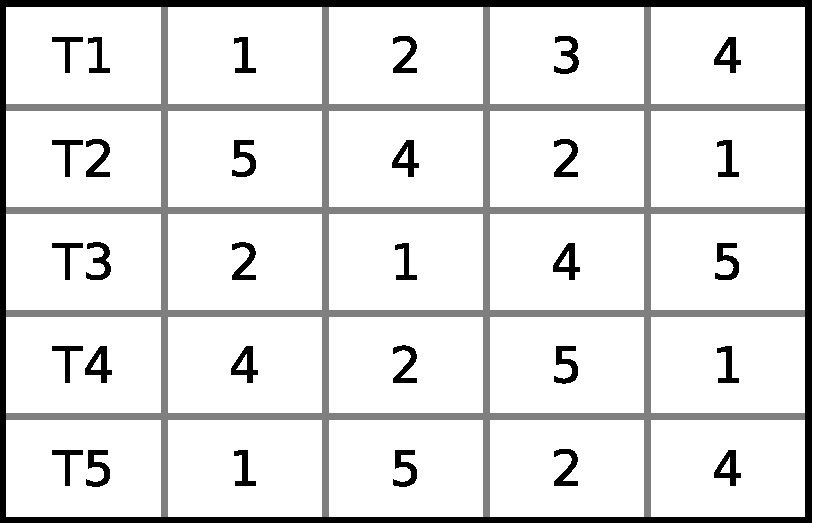
\includegraphics[scale=0.4]{pdf/validtrans}
\end{center}
\caption{Valid Transaction Dataset}
\label{Fig 1}
\end{figure}

\begin{figure}
\begin{center}
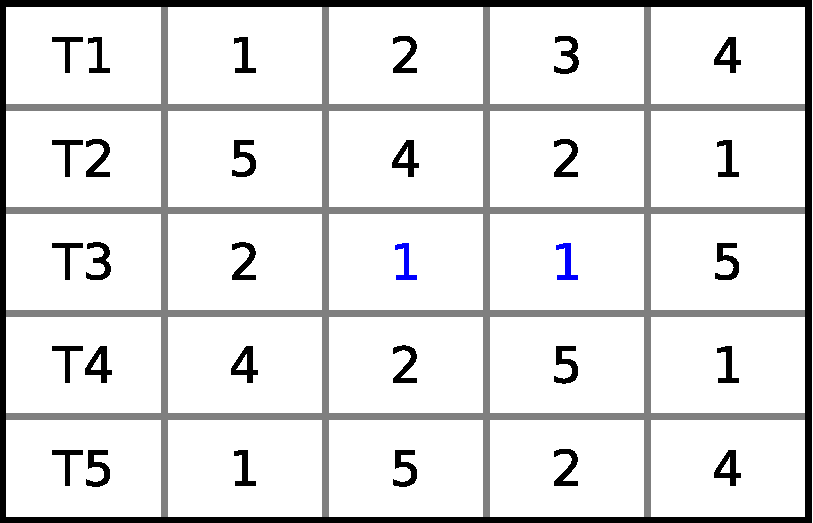
\includegraphics[scale=0.4]{pdf/invalidtrans}
\end{center}
\caption{Invalid Transaction Dataset}
\label{Fig 2}
\end{figure}

Transaction database \ref{Fig 1} is valid and \ref{Fig 2} is invalid(duplicate items(blue color) in \emph{T3}).

\item MASP


\end{enumerate}










In our scenario
Every transaction must contains equal number of items
In every transaction items must be unique

How to generate MASP tree?
How rules are extracted from MASP tree?

New approach: order independent + first occurence
How to generate multiple MASP tree
Many Rules obtained from MASP trees are discarded

Provide Definition of new terms

Apply Multiple Masp Tree and hence rules generation based on an example.
Provide algorithms


\section*{References}

\bibliography{mybibfile}

\end{document}